\documentclass{../../slides-style}

\slidetitle{Внутреннее представление данных}{27.09.2023}

\begin{document}
    
    \begin{frame}[plain]
        \titlepage
    \end{frame}
    
    \begin{frame}
        \frametitle{Побитовые операции}
        \begin{columns}
            \begin{column}{0.6\textwidth}
                \begin{itemize}
                    \item \& --- побитовое ``И''
                    \item | --- побитовое ``ИЛИ''
                    \item $\sim$ --- побитовое ``НЕ''
                    \item 1 \& 2 == false, но 1 \&\& 2 == true
                    \item $<<$, $>>$ --- битовый сдвиг
                    \begin{itemize}
                        \item int x = 1 $<<$ 3
                    \end{itemize}
                    \item sizeof --- размер типа в байтах
                    \begin{itemize}
                        \item int s = sizeof(int) * 8
                    \end{itemize}
                    \item Обратите внимание, что ВСЁ хранится как набор бит
                    \begin{itemize}
                        \item ``3'' --- литерал, лишь удобная форма записи 00...0011 в коде
                    \end{itemize}
                \end{itemize}
            \end{column}
            \begin{column}{0.4\textwidth}
                Маски
                \vspace{3mm}
                \begin{textblock}{1}(-0.35,0.4)
                    \&
                \end{textblock}
                \begin{tabu} {| X[1 l p] | X[1 l p] | X[1 l p] | X[1 l p] | X[1 l p] | X[1 l p] | X[1 l p] | X[1 l p] |}
                    \tabucline-
                    \everyrow{\tabucline-}
                    1 & 1 & 0 & 1 & 1 & 0 & 1 & 0 \\
                    0 & 0 & 0 & 0 & 0 & 0 & 0 & 1 \\
                    0 & 0 & 0 & 0 & 0 & 0 & 0 & 0 \\
                \end{tabu}
                \vspace{0.5cm}

                \begin{textblock}{1}(-0.35,0.4)
                    \&
                \end{textblock}
                \begin{tabu} {| X[1 l p] | X[1 l p] | X[1 l p] | X[1 l p] | X[1 l p] | X[1 l p] | X[1 l p] | X[1 l p] |}
                    \tabucline-
                    \everyrow{\tabucline-}
                    1 & 1 & 0 & 1 & 1 & 0 & 1 & 0 \\
                    0 & 0 & 0 & 0 & 0 & 0 & 1 & 0 \\
                    0 & 0 & 0 & 0 & 0 & 0 & 1 & 0 \\
                \end{tabu}
            \end{column}
        \end{columns}
    \end{frame}

    \begin{frame}[fragile]
        \frametitle{Работа с масками}
        \begin{footnotesize}
            \begin{minted}{cpp}
char x = 5;

int bit = 0b10000000;
for (int j = 0; j < 8; ++j)
{
    printf((x & bit) ? "1" : "0");
    bit = bit >> 1;
}
            \end{minted}
        \end{footnotesize}
    \end{frame}

    \begin{frame}
        \frametitle{Целые числа}
        \begin{itemize}
            \item Прямой код
            \begin{itemize}
                \item $5$ --- $00000101$, $-5$ --- $10000101$
            \end{itemize}
            \item Дополнительный код
            \begin{itemize}
                \item $5$ --- $00000101$, $-5$ --- $11111011$
                \item $-x$ представляется как $2^n - x$, поэтому и дополнительный
                \begin{itemize}
                    \item $n$ --- разрядность регистра
                    \item Можно понимать как ``старший разряд имеет вес $-2^{n-1}$''
                    \item Старший разряд всегда 1 для отрицательных чисел
                \end{itemize} 
                \item При сложении единица переноса в старшем разряде отбрасывается
            \end{itemize}
        \end{itemize}
    \end{frame}

    \begin{frame}
        \frametitle{Как это можно представлять}
        \begin{center}
            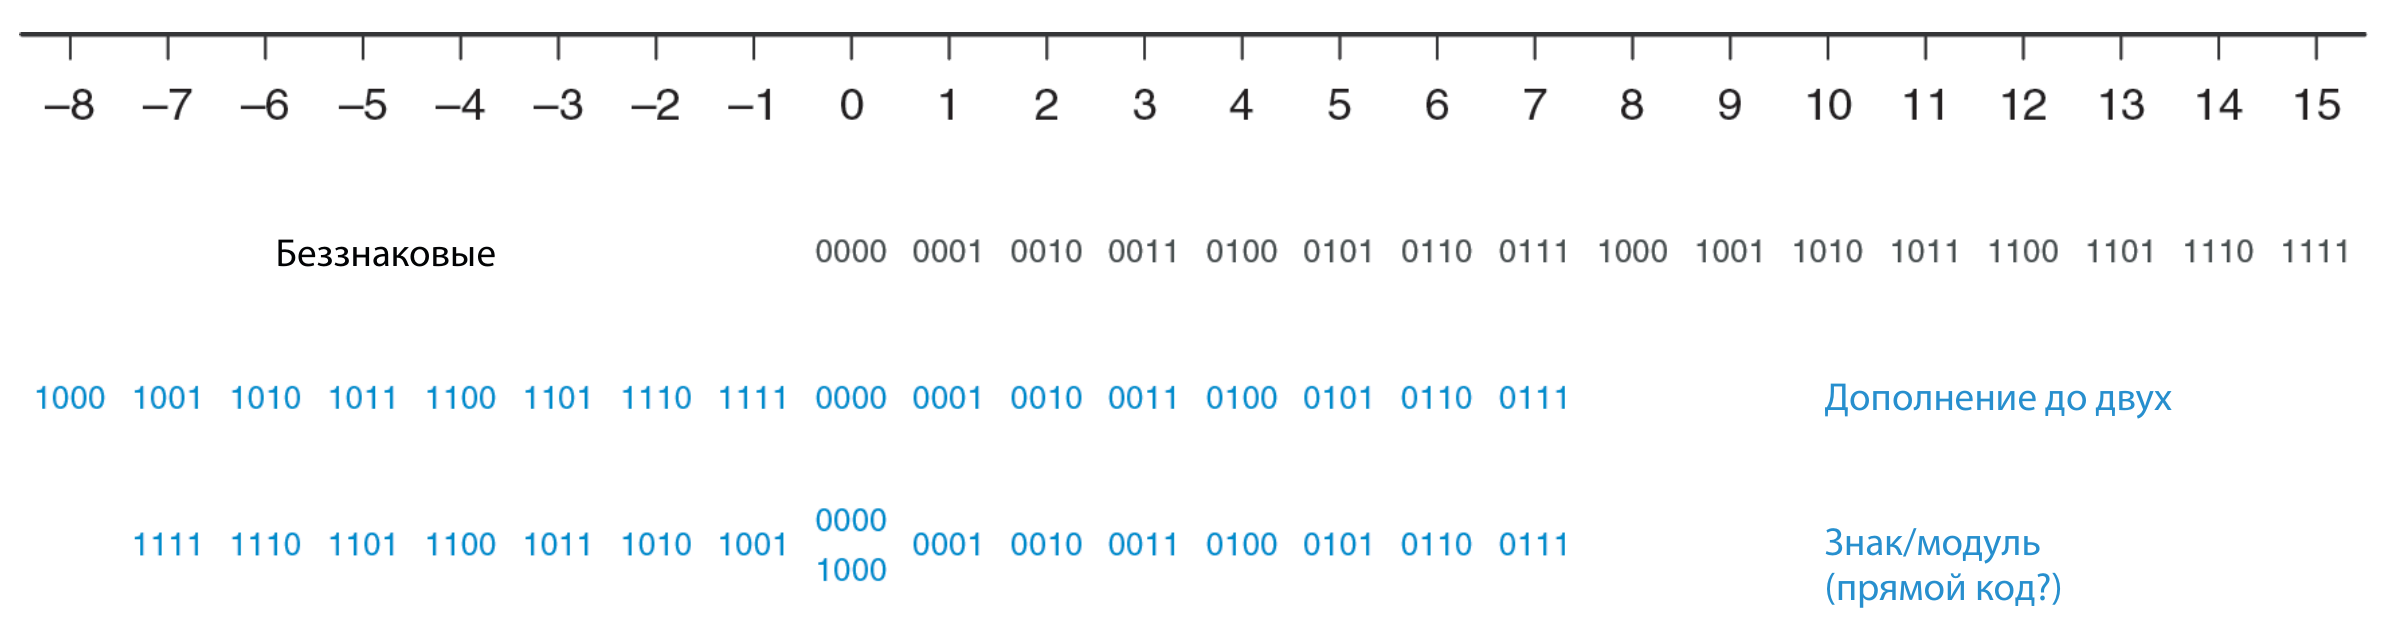
\includegraphics[width=\textwidth]{integerScale.png}
            \attribution{Д.М. Харрис, С.Л. Харрис, Цифровая схемотехника и архитектура компьютера RISC-V}
        \end{center}
    \end{frame}

    \begin{frame}[fragile]
        \frametitle{Формат записи}
        \begin{itemize}
            \item Литералы
            \begin{itemize}
                \item \mintinline{cpp}|int hexadecimal = 0x35FF;|
                \item \mintinline{cpp}|int octal = 03567;|
                \item \mintinline{cpp}|int binary = 0b00100111;|
                \item \mintinline{cpp}|0xFF == 255|
            \end{itemize}
            \item 
            \begin{footnotesize}
                \begin{minted}{cpp}
int x = 239;
unsigned char *b = (unsigned char*)(&x);
printf("0x%02X%02X%02X%02X\n", b[0], b[1], b[2], b[3]);
                \end{minted}
            \end{footnotesize}
        \end{itemize}
        \begin{center}
            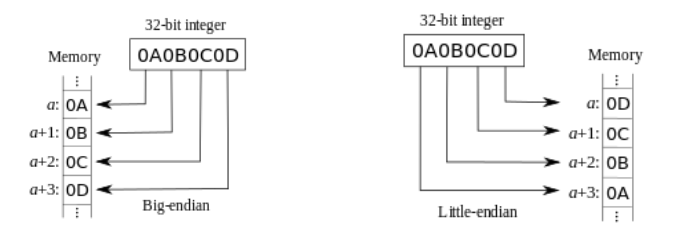
\includegraphics[width=0.8\textwidth]{little-endian-big-endian.png}
        \end{center}
    \end{frame}

    \begin{frame}
        \frametitle{Вещественные числа}
        \begin{itemize}
            \item IEEE 754 --- международный стандарт
            \item $x = (+-)m * p^q$
            \begin{itemize}
                \item p --- основание системы счисления
                \item q --- порядок числа (целое число)
                \item m --- мантисса числа (правильная p-ичная дробь, у которой первая цифра после запятой не равна 0)
                \begin{itemize}
                    \item Часто используют нормализованную запись, $m \in [1, p)$
                \end{itemize}
                \item Например:
                \begin{itemize}
                    \item $3,1415926 = 0, 31415926 * 10^1$
                    \item $1000=0,1 * 10^4$
                    \item $0,123456789 = 0,123456789 * 10^0$
                    \item $0,0000107_8 = 0,107_8 * 8^{-4}$
                    \item $1000,0001_2 = 0, 10000001_2 * 2^4$
                    \item $0 = 0,0 * 10^0$
                \end{itemize}
            \end{itemize}
        \end{itemize}
    \end{frame}

    \begin{frame}
        \frametitle{Внутреннее представление}
        \begin{itemize}
            \item $123.456$
            \item Наиболее точное представление (IEEE 754 Double, 64 бит): $1.23456000000000003069544618484E2$
            \begin{center}
                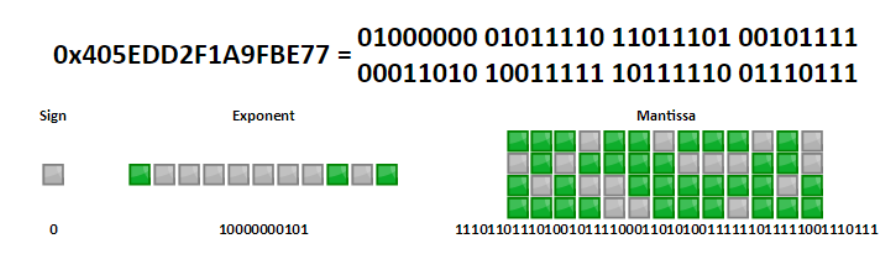
\includegraphics[width=0.8\textwidth]{internal-representation.png}
            \end{center}
            \item \url{http://www.binaryconvert.com/}
        \end{itemize}
    \end{frame}

    \begin{frame}
        \frametitle{Смещённый порядок}
        \begin{itemize}
            \item $123.456:  q = 10000000101_2???$
            \item Смещённый порядок =  $2^{a - 1} - 1$ + <истинный порядок>
            \begin{itemize}
                \item a --- количество разрядов, отводимых под порядок
                \item Чтобы не хранить знак ещё и порядка числа
            \end{itemize}
            \item $123.456 \approx 1111011.01110100101111 = 1.11101101110100101111 * 2^6$
            \item Смещённый порядок = $2^{10} - 1 + 6 = 1029_{10} = 10000000101_2$
        \end{itemize}
    \end{frame}

    \begin{frame}[fragile]
        \frametitle{Специальные числа}
        \begin{columns}
            \begin{column}{0.6\textwidth}
                \begin{itemize}
                    \item Неопределённость (NaN):
                    \begin{center}
                        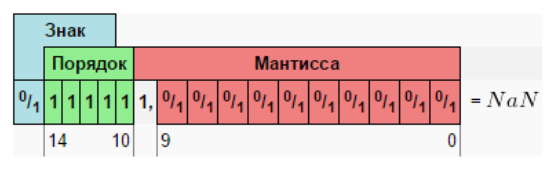
\includegraphics[width=0.8\textwidth]{nan.png}
                    \end{center}
                    \item Бесконечности:
                    \begin{center}
                        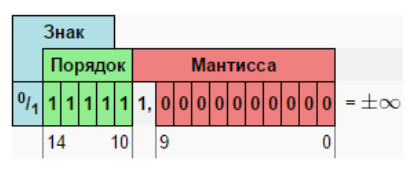
\includegraphics[width=0.8\textwidth]{infinity.png}
                    \end{center}
                \end{itemize}
            \end{column}
            \begin{column}{0.4\textwidth}
                \begin{footnotesize}
                    \begin{minted}{cpp}
double y = 0.0;
double x = 239.0 / y;
printf("%f", x);
                    \end{minted}
                \end{footnotesize}
            \end{column}
        \end{columns}
    \end{frame}

    \begin{frame}
        \frametitle{Строки}
         Строка как последовательность символов (их кодов) --- таблица символов
            \begin{itemize}
                \item ASCII (American Standard Code for Information Interchange)
                \begin{itemize}
                    \item 8 бит на символ (0 -- 255), 0 -- 127 стандартны, 128 -- 255 --- для локальных алфавитов
                    \item Кодовые страницы
                    \begin{itemize}
                        \item cp866
                        \item cp1251
                        \item koi8-r
                        \item ...
                    \end{itemize}
                \end{itemize}
                \item Unicode
            \end{itemize}
            Строка как последовательность байт --- кодировка
            \begin{itemize}
                \item UCS-16BE, UCS16-LE, UTF-8
            \end{itemize}
    \end{frame}

    \begin{frame}
        \frametitle{Зачем}
        \begin{itemize}
            \item Локализация --- перевод программы на другой язык (и под другую культуру)
            \item Интернационализация --- сделать так, чтобы программу было можно локализовать
            \item У однобайтовых кодировок некоторые проблемы с иероглифическими языками
            \begin{itemize}
                \item Shift JIS и прочие странные вещи
            \end{itemize}
        \end{itemize}
    \end{frame}

    \begin{frame}
        \frametitle{Локаль}
        \begin{itemize}
            \item Функция setlocale
            \item Категории: 
            \begin{itemize}
                \item LC\_COLLATE --- сравнение строк (strcoll)
                \item LC\_CTYPE --- типы символов 
                \item LC\_MONETARY --- формат денежных сумм
                \item LC\_NUMERIC --- десятичный разделитель и числа
                \item LC\_TIME --- формат времени (strftime)
                \item LC\_ALL --- всё
            \end{itemize}
            \item Имя локали, тэг языка (ru-RU), ищется в таблицах
            \item Локаль C, пустая локаль
            \item .code page --- указать кодовую страницу явно
            \item Пример: \mintinline{c}{setlocale(LC_ALL, "Ru.866");}
            \item Visual Studio использует по умолчанию кодировку 1251, консоль --- 866
            \item Под Linux --- UTF-8
        \end{itemize}
    \end{frame}

    \begin{frame}
        \frametitle{Юникод}
        \begin{itemize}
            \item UCS, universal character set
            \begin{itemize}
                \item Кодовые позиции --- целые числа (U+0000 – U+007F, …)
                \item Порядка 110 000 кодовых позиций
            \end{itemize}
            \item UTF, Unicode transformation format
            \begin{itemize}
                \item Кодировки --- битовое представление кодов из UCS
            \end{itemize}
            \item UTF-8
            \begin{itemize}
                \item 0x00000000 -- 0x0000007F: 0xxxxxxx
                \item 0x00000080 -- 0x000007FF: 110xxxxx 10xxxxxx
                \item 0x00000800 -- 0x0000FFFF: 1110xxxx 10xxxxxx 10xxxxxx
                \item 0x00010000 -- 0x001FFFFF: 11110xxx 10xxxxxx 10xxxxxx 10xxxxxx
                \item В точности совпадает с ASCII для первых 127 символов
            \end{itemize}
            \item BOM (Byte Order Mark)
            \begin{itemize}
                \item FE FF, FF FE, EF BB BF
            \end{itemize}
        \end{itemize}
    \end{frame}

\end{document}

